\documentclass[pdf,compress]{beamer}
\mode<presentation>{}
\usepackage{lmodern}
\usepackage[normalem]{ulem}
\usepackage[final]{pdfpages}
\usepackage[czech]{babel}
\usepackage[T1]{fontenc}
\usepackage[utf8x]{inputenc}
\usepackage{hyperref} % urls support, usage: \hyperref[label_name]{''link text''}
\usepackage{tikz} % for images positioning
\usetikzlibrary{backgrounds}

\usepackage{moreverb}

\addto\captionsczech{% Replace "english" with the language you use
  \renewcommand{\contentsname}%
    {Contents}%
    }


%apply styling
%use with \input at the beginning of all presentations

\usetheme[subsection=false]{Dresden}

\setbeamertemplate{navigation symbols}{}

\definecolor{SWIOrangeDark}{RGB}{249, 157, 28} % SWI logo orange color
\definecolor{SWIGray}{RGB}{68, 68, 68} % SWI logo gray color
\definecolor{SWIOrangeLight}{RGB}{251, 188, 102} % lighter orange
\definecolor{SWIGreyLight}{RGB}{108, 108, 108} % lighter grey

\setbeamercolor{palette primary}{bg=SWIGray,fg=SWIOrangeDark}
\setbeamercolor{palette secondary}{bg=SWIGray,fg=SWIOrangeDark}
\setbeamercolor{palette tertiary}{bg=SWIGray,fg=SWIOrangeDark}
\setbeamercolor{palette quaternary}{bg=SWIGray,fg=SWIOrangeDark}
\setbeamercolor{structure}{fg=SWIOrangeDark} % itemize, enumerate, etc
\setbeamercolor{section in toc}{fg=SWIOrangeDark} % TOC sections

% Override palette coloring with secondary
\setbeamercolor{subsection in head/foot}{bg=SWIGreyLight,fg=white}

\setbeamertemplate{footline}
{
  \leavevmode%
  \hbox{%
    \begin{beamercolorbox}[wd=.8\paperwidth,ht=2.25ex,dp=1ex,left]{bg=black,fg=title in head/foot}%
\hspace*{3ex}    \insertframenumber{} / \inserttotalframenumber\hspace*{1ex}
  \end{beamercolorbox}%
  \begin{beamercolorbox}[wd=.2\paperwidth,ht=2.25ex,dp=1ex,center]{bg=black,fg=title in head/foot}%
%
\includegraphics[height=0.5cm]{../shared/SW_Logo_md.png} \hspace*{1ex}%
  \end{beamercolorbox}%

  }
  \vskip0pt%
}%


\AtBeginSection[]
{
\setbeamercolor{section in toc}{fg=SWIOrangeDark}
\setbeamercolor{section in toc shaded}{fg=structure}
\begin{frame}<beamer>
  \frametitle{Contents}
  \tableofcontents[currentsection, hideallsubsections]
\end{frame}
}

\makeatother
\makeatletter


\title{Tooling for Java EE applications}
\subtitle{PA165}
\date{26.\,9.\,2017}
\author{Jiří Uhlíř, Martin Kotala}
%\institute{Fakulta informatiky, Masarykova univerzita}

\begin{document}
\frame{\titlepage}

\section[]{}
\begin{frame}
\frametitle{Contents}
\tableofcontents[hideallsubsections]
\end{frame}








\section[Git Basics]{Git Basics}
\subsection[]{Version control}
\begin{frame}
\frametitle{Version control}
\begin{itemize}
	\item Motivation
	\item History
		\begin{itemize}
		\item One file at a time
		\item Centralized (CVS, Subversion)
		\item Distributed (Git, Mercurial)
		\end{itemize}
\end{itemize}
\end{frame}

\subsection[]{Git history}
\begin{frame}
\frametitle{Git history}
\begin{itemize}
	\item Created in 2005 by Linus Torvalds 
		\begin{itemize}
		\item described by himself as "stupid content tracker"
		\item Originally created for linux kernel development
		\end{itemize}
	\item Inspired by BitKeeper, aiming to be performant and free
	\item CVS taken as example of what \textit{not to do}
	\item git - no exact meaning
		\begin{itemize}
		\item random three-letter combination that is pronounceable, and not actually used by any common UNIX command. The fact that it is a mispronunciation of "get" may or may not be relevant.
		\item "global information tracker": you're in a good mood, and it actually works for you. Angels sing, and a light suddenly fills the room.
		\item "g*dd*mn idiotic truckload of sh*t": when it breaks
		\item \url{https://github.com/git/git/blob/master/README.md} 
		\end{itemize}	
\end{itemize}
\end{frame}



\subsection[]{Git characteristicsl}
\begin{frame}
\frametitle{Git characteristics}
\begin{itemize}
	\item Strong support for non-linear development
	%Git supports rapid branching and merging, and includes specific tools for visualizing and navigating a non-linear development history. In Git, a core assumption is that a change will be merged more often than it is written, as it is passed around to various reviewers. In Git, branches are very lightweight: a branch is only a reference to one commit. With its parental commits, the full branch structure can be constructed.
		\begin{itemize}
		\item Rapid branching and merging
		\item Tools for visualisation and navigation in development history
		\item Lightweight branches % branch = reference to only one commit
		\end{itemize}
	\item Distributed development
	%Like Darcs, BitKeeper, Mercurial, SVK, Bazaar, and Monotone, Git gives each developer a local copy of the full development history, and changes are copied from one such repository to another. These changes are imported as added development branches, and can be merged in the same way as a locally developed branch.
		\begin{itemize}
		\item Each developer has full history
			\begin{itemize}
			\item Prevents data loss
			\item Subteams can share reposities without access to central repository
			\end{itemize}
		\item No need to have access to central repository all the time
		\item Changes are commited locally and then pushed to central repository
		\end{itemize}%TODO anything else?
\end{itemize}
\end{frame}

\begin{frame}
\frametitle{Git characteristics}
\begin{itemize}
	\item Variety of protocols supported
	%Repositories can be published via Hypertext Transfer Protocol (HTTP), File Transfer Protocol (FTP), rsync (removed in Git 2.8.0[31]), or a Git protocol over either a plain socket, or Secure Shell (ssh). Git also has a CVS server emulation, which enables the use of extant CVS clients and IDE plugins to access Git repositories. Subversion and svk repositories can be used directly  with git-svn.
		\begin{itemize}
		\item HTTP/HTTPS
		\item FTP
		\item SSH %using passkey without need to provide username/pass
		\end{itemize}
	\item Efficient handling of large projects
	%Torvalds has described Git as being very fast and scalable,[32] and performance tests done by Mozilla[33] showed it was an order of magnitude faster than some version control systems, and fetching version history from a locally stored repository can be one hundred times faster than fetching it from the remote server.[34]
		\begin{itemize}
		\item Fast (when applying patches)
		\item Scalable
		\item Fetching version history from locally stored repository is faster then from remote
		\end{itemize}%TODO anything else?
	\item Allows various workflows
		\begin{itemize}
		\item Centralized (enterprise companies)
		\item Hierarchical (Linux kernel)
		\item Distributed (open source projects, pull requests)
		\end{itemize}%TODO anything else?
\end{itemize}
\end{frame}

% Ok, that was enough for theory
\subsection[]{Git locally}
\begin{frame}
\frametitle{Git Basics - commands}

\textbf{git init}
	\begin{itemize}
	\item Initializes empty local repository
	\end{itemize}
\textbf{git status}
	\begin{itemize}
	\item Shows current file differences between HEAD commit and current working copy
	\end{itemize}
\textbf{git add <filename>}
	\begin{itemize}
	\item Adds a file/directory into commit checklist
	\item -A (all files not versioned, or not ignored), -u (only updated files already under version control)
	\end{itemize}
\textbf{git commit -m <message>}
	\begin{itemize}
	\item Records working copy changes into repository
	\end{itemize}
\end{frame}

\begin{frame}
\frametitle{Git Basics - commands}

\textbf{git log}
	\begin{itemize}
	\item Shows latest commits for local repository
	\item -{}-oneline (condensed view), -{}-graph (includes branches)
	\end{itemize}
\textbf{git diff}
	\begin{itemize}
	\item Shows code difference between HEAD commit and current working copy
	\end{itemize}
\textbf{git checkout / git reset}
	\begin{itemize}
	\item Removes local uncommited changes
	\end{itemize}
\textbf{git reset -{}-soft HEAD~1 / -{}-hard <commithash>}
	\begin{itemize}
	\item Reverts working copy to given commit (soft keeps changes as \emph{to be commited}, hard removes them completely)
	\end{itemize}
\textbf{git tag}
	\begin{itemize}
	\item Annotates current version of local repository with tag (such as version)
	\end{itemize}
\end{frame}

\begin{frame}
\frametitle{Git Basics - commands}
\textbf{git clone}
	\begin{itemize}
	\item Clones remote repository into local repository and fetches latest changes
	\end{itemize}
\textbf{git push}
	\begin{itemize}
	\item Pushes local commited changes into remote repository
	\item -{}-tags Pushes tags into remote repository
	\item Cleanup local commits before push using amend or rebase
	\end{itemize}
\textbf{.gitignore}
	\begin{itemize}
	\item File for specifying files not to be tracked under version control (binary files, log files, temporary build files, etc.)
	\end{itemize}
\textbf{.gitattributes}
	\begin{itemize}
	\item File for specifying attributes to apply for certain paths
	\item Used for example for specifying line endings
	\end{itemize}
\end{frame}




\subsection[]{Git Basics - Demo}
\begin{frame}
\frametitle{Git Basics - Demo}
\end{frame}






%\section[Git Branching]{Git Branching}
\subsection[]{Overview}
\begin{frame}
\frametitle{Git Branching - Overview}
\begin{itemize}
	\item A branch represents an independent line of development.
	\item Lightweight implementation of branching – Git stores a branch as \textbf{a reference to a commit}.
	\item Keeps history as a tree, where \textbf{each commit is a node} in the tree, and has one or more parents.
	\item History is \textbf{extrapolated through the commit relationships}.
	\item It’s a good practice to \textbf{spawn a new branch to encapsulate your changes} no matter how big the changes are.
\end{itemize}
\end{frame}



\subsection[]{Local Branches}
\begin{frame}
\frametitle{Git Branching - Local Branches}
\begin{itemize}
	\item \textbf{Non-tracking local branches}
		\begin{itemize}
		\item Exist on user’s machine.
		\item Not associated with any other branch.
		\item User needs to specify which upstream branch when running push or pull commands.
		\end{itemize}
	\item \textbf{Tracking local branches}
		\begin{itemize}
		\item Exist on user’s machine.
		\item Tracking branch is a branch that has a direct relationship to another branch.
		\item Local tracking branches in most cases track a remote tracking branch.
		\item Allow user to run git pull and git push without specifying which upstream branch to use.
		\end{itemize}
\end{itemize}
\end{frame}

\subsection[]{Local Branches - remote-tracking branches}
\begin{frame}
\frametitle{Git Branching - remote-tracking branches}
\begin{itemize}
	\item \textbf{Remote}
		\begin{itemize}
		\item Remote connection (bookmark) into other repository.
		\end{itemize}
	\item \textbf{Remote branch}
		\begin{itemize}
		\item Branch on a remote location.
		\end{itemize}
	\item \textbf{Remote-tracking branch}
		\begin{itemize}
		\item Local cache for what the remote repositories contain.
		\item (remote)/(branch)
			\begin{itemize}
			\item origin/master
			\item origin/test-branch
			\end{itemize}
		\end{itemize}
	\item \textbf{Note:}
		\begin{itemize}
		\item “origin” and “master” are not special.
		\end{itemize}
\end{itemize}
\end{frame}

\subsection[]{Git Branching - merge}
\begin{frame}
\frametitle{Git Branching - merge}
\begin{itemize}
	\item Way of putting a forked \textbf{history back together} again.
	\item\textbf{Non-destructive} operation.
	\item All the operations always \textbf{merge into the current} branch.
	\item Git has \textbf{several distinct algorithms} to accomplish the merge.
\end{itemize}
Note:
\begin{itemize}
	\item git pull command effectively runs git fetch and git merge.
\end{itemize}
\end{frame}

\begin{frame}
\frametitle{Git Branching - merge}
\begin{itemize}
	\item \textbf{3-Way Merge}
		\begin{itemize}
		\item Creates \textbf{merge commit} that ties together the histories of both branches.
		\item Merge commit as a \textbf{symbolic joining} of the two branches.
		\item Original \textbf{context is maintained}.
		\end{itemize}
	\item \textbf{Fast-Forward Merge}
		\begin{itemize}
		\item Requires \textbf{linear path} from the current branch tip to the target branch.
		\item Usually \textbf{facilitated through rebasing} – suitable for small tasks and fixes.
		\item Context of the affected commits as part of an earlier feature branch is lost.
		\end{itemize}
\end{itemize}
\end{frame}

\subsection[]{Git Branching - 3-way merge}
\begin{frame}
\frametitle{Git Branching - 3-way merge}
\begin{tikzpicture}
  \node (img1) {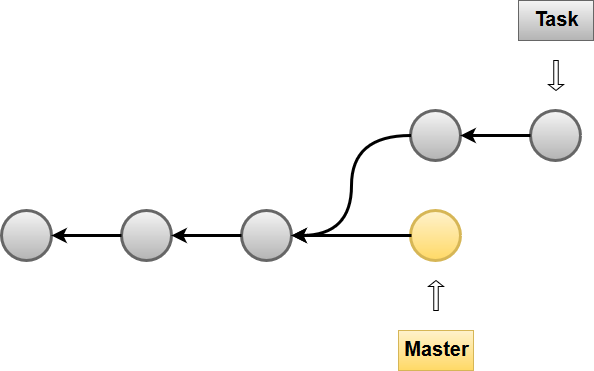
\includegraphics[width=6.4cm, height=4cm]{3waymerge-1.png}};
%  \pause
  \begin{scope}[on background layer]
  	\node (img2) at (img1.south east) [yshift=-1cm] {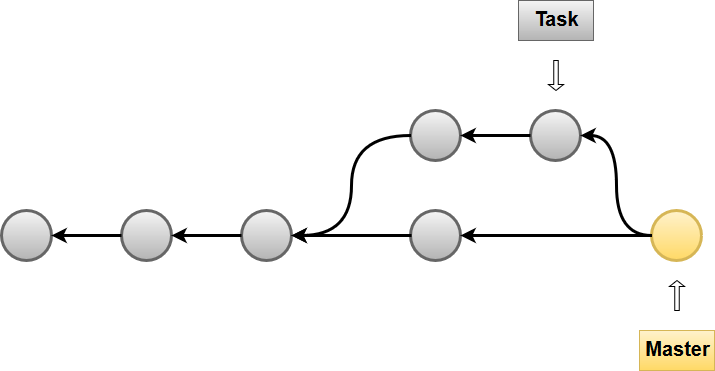
\includegraphics[width=7.7cm, height=4cm]{3waymerge-2.png}};
  \end{scope}
\end{tikzpicture}
\end{frame}

\subsection[]{Git Branching - fast-forward merge}
\begin{frame}
\frametitle{Git Branching - fast-forward merge}
\begin{tikzpicture}
  \node (ffwd1) {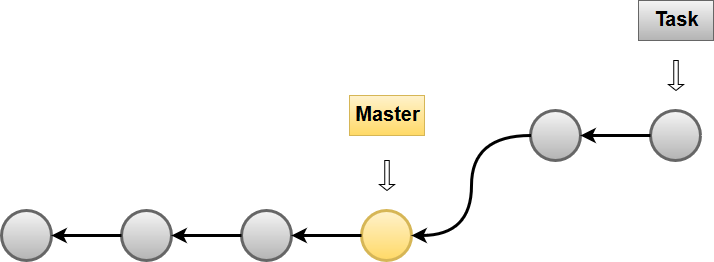
\includegraphics[width=8.18cm, height=3cm]{fastfwd-1.png}};
%  \pause
  \begin{scope}[on background layer]
  	\node (ffwd2) at (ffwd1.south east) [yshift=-1.5cm, xshift=-2cm] {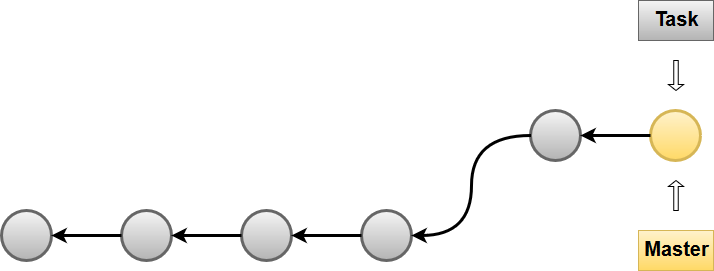
\includegraphics[width=7.9cm, height=3cm]{fastfwd-2.png}};
  \end{scope}
\end{tikzpicture}
\end{frame}

\subsection[]{Git Branching - rebase}
\begin{frame}
\frametitle{Git Branching - rebase}
\begin{itemize}
	\item Process of \textbf{moving or combining} a sequence of commits to a new base commit – alternative to merge.
	\item Makes the branch appear as if you'd created it from a different commit.
	\item Git takes changes from your branch and \textbf{replays them} on top of the destination branch.
	\item Result branch \textbf{looks the same} but it's composed of entirely new commits.
	\item Do not rebase commits that exist \textbf{outside your repository} (unless you have a good reason to do so).
\end{itemize}
\end{frame}

\begin{frame}
\frametitle{Git Branching - rebase}
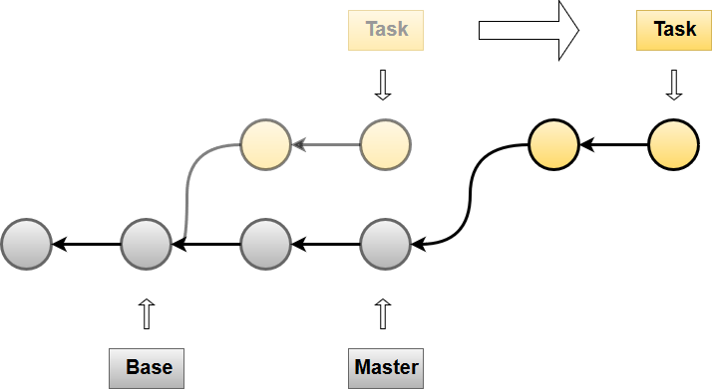
\includegraphics[width=\textwidth, height=0.55\textwidth]{rebase.png}
\end{frame}

\begin{frame}
\frametitle{Git Branching - rebase}
\begin{itemize}
	\item Rebase helps to maintain a \textbf{linear project history} – that allows an easier investigation of regression issues.
	\item \textbf{Workflow example:}
		\begin{enumerate}
		\item User creates the new task branch from master and starts working in it.
		\item There is an active development on a master branch.
		\item User wants to get the latest updates from master to task branch.
		\item User performs regular rebase operation to move his commits on top of latest master commits.
		\item User is done with his task and performs the final rebase and merge to master.
		\item Git is able to apply fast-forward algorithm for the merge.
		\end{enumerate}
\end{itemize}
\end{frame}

\begin{frame}
\frametitle{Git Branching - rebase}
\begin{itemize}
	\item \textbf{Interactive rebase}
		\begin{itemize}
		\item Allows user to \textbf{alter individual commits} in the process of rebasing.
		\item Support for powerful \textbf{history rewriting} features.
		\item Useful for history cleanup: reword, edit, squash, fixup
		\item Always amend commits that have \textbf{not been pushed} yet to avoid confusion.
		\end{itemize}
\end{itemize}
\end{frame}

\subsection[]{Git Branching - conflicts}
\begin{frame}
\frametitle{Git Branching - conflicts}
\begin{itemize}
	\item Conflicts may occur during merge and rebase operations.
	\item Use the suitable \textbf{merge strategy} to avoid conflicts.
	\item When the conflict occurs:
		\begin{itemize}
		\item \textbf{Abort} the merge with.
		\item \textbf{Work through} the conflict and \textbf{continue}.
		\end{itemize}
	\item \textbf{Visualize and resolve} conflict in merge tool.
\end{itemize}
Note:
\begin{itemize}
	\item Rebase has an option to \textbf{skip/bypass} conflicting commit.
\end{itemize}
\end{frame}

\subsection[]{Git Branching - commands}
\begin{frame}
\frametitle{Git Branching - commands}
\textbf{git branch}
	\begin{itemize}
	\item List all of the branches in your repository.
	\end{itemize}
\textbf{git branch <new-branch-name>}
	\begin{itemize}
	\item Create a new branch called <new-branch-name>.
	\end{itemize}
\textbf{git branch -d <existing-branch-name>}
	\begin{itemize}
	\item Delete the existing branch, safely. Use –D to force it.
	\end{itemize}
\textbf{git checkout <existing-branch-name>}
	\begin{itemize}
	\item Navigate between the existing branches.
	\end{itemize}
\textbf{git checkout -b <new-branch-name> <remote>/<branch-name>}
	\begin{itemize}
	\item Create and checkout a new local tracking branch.
	\item Or simply use the previous command if there is only one remote tracking branch called <branch-name>. This applies to Git 1.6.6+. 
	\end{itemize}
\end{frame}


\begin{frame}
\frametitle{Git Branching - commands}
\textbf{git remote}
	\begin{itemize}
	\item List the connections to remote repositories. Use -v to get URLs. 
	\end{itemize}
\textbf{git remote add <remote-name> <url>}
	\begin{itemize}
	\item Add a new connection to a remote repository.
	\end{itemize}
\textbf{git remote rm <remote-name>}
	\begin{itemize}
 	\item Remove the connection to a remote repository.
	\end{itemize}
\textbf{git fetch <remote-name>}
	\begin{itemize}
	\item Fetch all of the branches from the remote repository.
	\end{itemize}
\textbf{git pull <remote-name>}
	\begin{itemize}
	\item Fetch the remote’s copy of the current branch and merge it into the local copy.
	\end{itemize}
\textbf{git push <remote-name> <branch-name>}
	\begin{itemize}
	\item Push the specified branch to remote repository
	\end{itemize}
\end{frame}

\begin{frame}
\frametitle{Git Branching - commands}
\textbf{git merge <existing-branch-name>}
	\begin{itemize}
	\item Merge the specified branch into current one and let Git to choose an algorithm.
	\end{itemize}
\textbf{git merge --no-ff <existing-branch-name>}
	\begin{itemize}
	\item Merge the specified branch into current one and generate merge commit.
	\end{itemize}
\textbf{git merge --ff-only <existing-branch-name>}
	\begin{itemize}
	\item Merge the specified branch into current one and refuse to merge when fast-forward is not possible.
	\end{itemize}
\textbf{git checkout task}
\textbf{git rebase master}
	\begin{itemize}
	\item Move the entire task branch to begin on the tip of the master branch, effectively incorporating all of the new commits in master.
	\end{itemize}
\end{frame}

\section[Pull requests]{Pull requests}
\subsection[]{Pull Requests - overview}
\begin{frame}
\frametitle{Pull Requests - overview}
\begin{itemize}
	\item Mechanism for a developer to \textbf{notify coworkers.}
	\item \textbf{Not a Git feature}, functionality provided by e.g. Bitbucket or GitHub.
	\item Interface for \textbf{discussing proposed changes} before integrating them into the official project code base.
	\item \textbf{4 pieces} of information:
		\begin{itemize} 
		\item source repository
		\item source branch
		\item destination repository
		\item destination branch
		\end{itemize}
\end{itemize}
\end{frame}

\subsection[]{Pull Requests - workflow}
\begin{frame}
\frametitle{Pull Requests - workflow}
\begin{enumerate}
	\item \textbf{Developer creates task/feature branch} to deliver the code.
	\item Once done the \textbf{developer pushes his dedicated local branch} to public repository.
	\item \textbf{Pull requests is created} (it’s good idea to rebase first).
	\item Coworkers \textbf{review the code} and provide feedback.
	\item Once approved the project maintainer \textbf{merges the changes.}
\end{enumerate}
\end{frame}


 



\end{document}
